\documentclass{article}

% Márgenes.
\usepackage{geometry}
\addtolength{\hoffset}{-0.2cm}
\addtolength{\textwidth}{0.4cm}
\addtolength{\voffset}{-0.5cm}
\addtolength{\textheight}{1cm}

% Caracteres especiales del español.
\usepackage[utf8]{inputenc}

% Para el lenguaje español.
\usepackage[spanish]{babel}

% Símbolos matemáticos
\usepackage{amssymb}

% Binomio de Newton.
\usepackage{amsmath}

% Imágenes
\usepackage{graphicx}
\graphicspath{ {./img/} }

% Algoritmos
\usepackage[ruled,vlined,linesnumbered]{algorithm2e}

% Para que los figuras se queden en su lugar.
\usepackage{float}

% Macros.
\newcommand{\tbf}[1]{\textbf{#1}}

\newcommand{\tit}[1]{\textit{#1}}

\newcommand{\ttt}[1]{\texttt{#1}}

% Título y autor del reporte.
\title{Uso de la Heurística de Colonia de Hormigas para Resolver
       el Problema del Asignación Generalizado (GAP)}
\author{Carrasco-Ruiz Mauricio  \\
	maucarrui@ciencias.unam.mx  \\
        Universidad Nacional Autónoma de México (UNAM) \\
        Facultad de Ciencias \\
        Heurísiticas de Optimización Combinatoria \\
	}

% Fecha de hoy.
\date{\today} 

\begin{document}

    \maketitle

    \begin{abstract}
      El Problema de Asignación Generalizado es 
      un problema de optimización combinatoria en donde 
      no solo entra en efecto que buscamos minimizar 
      la función de costo sino también buscamos 
      que la solución sea factible: que ningún trabajador
      sobrepase su capacidad. Por ello se decidió utilizar
      la heurística de Optimización de Colonia de Hormigas
      (ACO). La implementación hecha en C++ siempre daba 
      resultados factibles para múltiples instancias del 
      problema, sin embargo no se alcanzó a llegar a una 
      solución óptima; pues la implementación que se hizo
      fue elitista desde un principio, remarcando de esta 
      manera la importancia de diversificar nuestras 
      soluciones al principio de la heurística.
    \end{abstract}

    \section{Introducción} \label{intro}
    El Problema de Asignación Generalizado (GAP) es un 
    problema de optimización combinatoria en donde dado un 
    número de trabajadores y un número de tareas, una 
    tarea puede ser asignada a un trabajador y esta 
    asignación implica cierta capacidad y costo para el 
    trabajador; por lo que no sólo buscamos minimizar el 
    costo de estas asignaciones sino también no sobrepasar 
    la capacidad de un trabajador.

    Descrito formalmente, tenemos las siguientes funciones: 
    \[ a: \mathbb{Z}^+ \times \mathbb{Z}^+ \rightarrow \mathbb{R} \]
    \[ c: \mathbb{Z}^+ \times \mathbb{Z}^+ \rightarrow \mathbb{R} \]
    \[ b: \mathbb{Z}^+ \rightarrow \mathbb{R} \]

    En donde la función $a(i, j)$ nos regresa la capacidad del 
    trabajador $i$ de hacer la tarea $j$, la función $c(i, j)$
    nos regresa el costo de que el trabajador $i$ haga la tarea
    $j$, y la función $b(i)$ nos regresa la capacidad que el 
    trabajador $i$ tiene.

    Además tenemos la siguiente función característica:
    
    \[ x(i, j) = 
         \begin{cases}
           1 & \text{si } i \text{ realiza la tarea } j \\
           0 & \text{en otro caso} \\
         \end{cases}
    \]
    
    Por ende, en el GAP lo que buscamos es minimizar la siguiente
    función:

    \[ costo = \sum_{i = 1}^n \sum_{j = 1}^m c(i, j) \cdot x(i, j) \]

    Donde además tenemos que asegurar que se cumplan las siguientes 
    condiciones para que la solución sea factible:

    \[ \forall i ( \sum_{j = 1}^m a(i, j) \cdot x(i, j) \leq b(i) ) \]
    \[ \forall j \exists i (x(i, j) = 1) \]

    Es decir, que ningún trabajador sobrepasa su capacidad y que 
    para toda tarea existe un trabajador que la realiza.

    \subsection{Colonia de Hormigas} \label{ACO}
    Para resolver este problema se decidió utilizar a la heurística
    conocida como Optimización de Colonia de Hormigas (\tit{Ant Colony
    Optimization, ACO}). 

    Propuesta por Marco Dorigo et al. al principio de los 90's, el 
    desarrollo de esta heurística se basó fuertemente  en el 
    comportamiento que tienen las hormigas para buscar comida y 
    regresarla a su colonia. Resultando en que aquellas hormigas que
    descubrieran un camino más corto para encontrar comida, regresarían 
    más rápido a su colonia, y como las hormigas dejan feromonas por 
    donde han pasado entonces las siguientes hormigas que salgan de 
    la colonia van a seguir con una mayor probabilidad el camino con 
    las feromonas más ``frescas'' (es decir, con la mayor cantidad de 
    feromonas); en otras palabras, van a seguir el camino más corto.

    De esta forma, nosotros podemos modelar el escenario anterior 
    por medio de una gráfica $G = (V, E)$ en donde las aristas 
    indicarían los caminos que pueden tomar las hormigas y los 
    vértices los estados a los que pueden llegar las hormigas. 
    Nótese que además las aristas tendrían pesos que nos indicarían
    la cantidad de feromonas que han dejado por ahí las hormigas.

    Y así, una fórmula para poder calcular la probabilidad de que 
    una hormiga en el vértice $i$ vaya al vértice $j$ dependiendo 
    de la cantidad de feromonas que hay en la arista $e = (i, j)$ 
    es:

    \begin{equation} \label{prob}
      P(e_{i, j}) = \frac{ \tau_{i,j} } { \sum_{k = 1}^{|V|} \tau_{i, k} }
    \end{equation}

    Donde $\tau_{i, j}$ nos dice la cantidad de feromonas que hay
    en la arista $e = (i, j)$.

    Ahora hay que ver de qué manera podemos actualizar el valor 
    de las feromonas dependiendo de qué tan buena fue la solución 
    que encontró la hormiga. Para ello, sea $s$ la solución que 
    encontró la hormiga y $T$ la trayectoria que tomó la 
    hormiga en la gráfica, podemos actualizar las feromonas de la 
    siguiente manera:

    \begin{equation} \label{update}
      \tau_{i, j} \leftarrow \tau_{i, j} + \frac{Q}{f(s)} \text{ si } e_{i, j} \in T
    \end{equation}

    Donde $Q \in \mathbb{Z}^+$ y $f(s)$ es la función de costo.
    Así, sólo las aristas por las que han pasado las hormigas se 
    verán afectadas.

    Y por último hay que mencionar que las feromonas, así como 
    en la vida real, se van a tener que evaporar en nuestra
    gráfica; pues de esta forma permitimos que nuestras 
    hormigas no se atasquen en una única solución, sino que
    tengan la libertad de volver a explorar otros caminos 
    después de un rato. Para lograr esto, lo que hacemos es: 

    \begin{equation} \label{evaporation}
      \tau_{i, j} \leftarrow (1 - p) \cdot \tau_{i, j} \text{ para toda } e_{i, j} \in E
    \end{equation}

    Donde $p \in (0, 1]$. Logrando de esta forma que 
    soluciones buenas siempre mantengan sus aristas con
    feromonas pues muchas hormigas las van a seguir y
    malas soluciones eventualmente irán desapareciendo
    pues muy pocas hormigas las van a seguir.

    \section{Desarrollo} \label{development}
    Toda la implementación de la heurística se llevo a cabo
    en el lenguaje de programación C++.

    El problema de optimización GAP lo podemos ver como una 
    gráfica bipartita completa, obteniendo así una gráfica 
    que puedan recorrer nuestras hormigas.

    \subsection{ Un recorrido en especial para gráficas bipartitas }
    
    La heurística ACO esta diseñada para que las hormigas
    puedan recorrer cualquier tipo de gráfica y puedan
    encontrar una buena solución a nuestro problema. Sin 
    embargo, para nuestro caso se decidió modificar un 
    poco el comportamiento de las hormigas, con la finalidad
    de facilitar la construcción de una solución sin 
    perder el comportamiento de las hormigas. La manera 
    en la que trabajan nuestras hormigas es la siguiente:

    Todas las hormigas empiezan en el vértice que representa
    a la primera tarea, sea $v_i$, y escogen aleatoriamente
    dependiendo de la cantidad de feromonas que haya en las 
    aristas adyacentes a la tarea, a un trabajador $v_j$. 
    Agregan entonces la arista $e_{i,j}$ a su solución 
    actual, y se mueven a la siguiente tarea. Repitiendo 
    este proceso con todas las tareas que haya en el problema.
    Resultando así en una solución que va a contener a todas
    las tareas; sin embargo, no hay nada que asegure que esta 
    solución vaya a ser factible.

    \subsubsection{ Alternativas para obtener soluciones factibles }
    Como se mencionó en la ecuación (\ref{prob}), una forma 
    sencilla de obtener la probabilidad de escoger a un 
    trabajador (en este caso la arista), puede ser dividir la 
    feromona de esa arista entre la suma de todas las demás que
    son adyacentes a la tarea; sin embargo, esto no nos da 
    información extra sobre si la solución que vamos construyendo 
    sigue siendo factible o no.

    Hay que tomar en cuenta que la ecuación (\ref{update}) 
    actualiza a las feromonas con respecto a la función de costo, 
    en este caso aún no se ve reflejada la capacidad de un trabajador
    ni si se sobrepaso o no en esta operación. Por lo que tenemos
    dos opciones para poder incluir a la capacidad dentro de las 
    decisiones de nuestras hormigas: Penalizar a las aristas que 
    esten contribuyendo a que un trabajador se este sobrepasando 
    de su capacidad ó que dentro de la probabilidad de que las 
    hormigas eligan a un trabajador se vea reflejado si ya 
    se sobrepaso al agregarle una tarea o no.

    \paragraph{Penalización}
    Sea $s$ la solución construida por una hormiga, supongamos que 
    esta solución hace que el trabajador $i$ se sobrepase de su 
    capacidad por un $n \%$. Entonces del $100 \%$ que contribuían
    las feromonas relacionadas con el trabajador a la solución, les 
    vamos a penalizar un $m \%$, donde $m$ es :

    \[ m \% = \begin{cases}
          100 \% & \text{ si } n \geq 100 \% \\
          n \%   & \text{ en otro caso }
       \end{cases}
    \]

    En otras palabras 
    
    \[ penalizacion \leftarrow (1 - m) \]

    Sin embargo, si son múltiples tareas las que contribuyen a 
    esta sobrecapacitación entonces no las deberíamos de penalizar
    a todas por igual, pues puede que haya alguna tarea que 
    contribuye básicamente nada a esta penalización mientras que 
    hay alguna otra que contribuye casi en un $100 \%$ a esto.
    Por ende es necesario ver cuánto contribuye cada tarea a 
    esta sobrecapacitación, lo cual lo hacemos la siguiente manera:

    \[ contribucion(i, j) = \frac{ a(i, j) } { \sum_{(i, k) \in s} a(i, k) } \]

    Y entonces la penalización a la arista $e_{i, j}$ se reduce a:
    \[ penelizacion_{i, j} = contribucion(i, j) \cdot penalizacion \]

    Así, la feromona se ve afectada de la siguiente manera:
    \[ \tau_{i, j} \leftarrow \tau_{i, j} \cdot penalizacion_{i, j} \]

    Consiguiendo de esta forma, que las aristas que hayan contribuido
    más a que un trabajador se sobrepasara sean penalizadas más bruscamente
    que aquellas que casi no contribuyeron en nada. Así, eventualmente
    las feromonas más fuertes serían aquellas en donde el trabajador es 
    capaz de realizar la tarea sin que sobrepase su capacidad; obteniendo 
    una solución factible.

    \paragraph{Probabilidad} Hacemos un pequeño cambio a la ecuación 
    \ref{prob} y ahora tenemos lo siguiente:

    \begin{equation} \label{n_update}
            P(e_{i, j}) = 
              \frac{ [\tau_{i,j}]^{\alpha} [\eta(c, (i, j))]^{\beta} } 
                   { \sum_{k = 1}^{|W|} [\tau_{k,j}]^{\alpha} [\eta(c, (k, j))]^{\beta} }
    \end{equation}

    Donde $W$ es el conjunto de trabajadores del problema, y la función
    $\eta(c, e)$ nos regresa la probabilidad de que la arista $e_{i, j}$
    sea agregada a la solución parcial $c$ dependiendo de la capacidad 
    del trabajador $i$ para hacer la tarea $j$, y si en caso de que agregar
    $e$ a $c$ termina en que el trabajador $i$ sobrepase su capacidad 
    entonces regresa 0. Y $\alpha$ y $\beta$ son enteros positivos.

    Con este método se puede dar la posibilidad de que una hormiga ya 
    tenga construida una solución parcial $c'$ pero no importa 
    que arista más agregue a la solución, esta va a resultar en una 
    solución no factible; por lo tanto, habrá hormigas que no 
    terminarán de construir soluciones completas. Las feromonas de 
    estas aristas por las que pasaron estas hormigas no se veran 
    actualizadas pues no contribuyen a la heurística, pero sí 
    se evaporarán.

    Consiguiendo de esta manera, que las hormigas que logren terminar 
    de construir una solución, siempre regresen al hormiguero 
    con una solución factible. Es importante recalcar que 
    eventualmente, las únicas aristas que van a quedar con feromonas
    van a ser aquellas que nos regresen soluciones factibles; así 
    eventualmente las hormigas empezaran a regresar soluciones 
    factibles.

    \subsection{ Estructura del proyecto }
    Ahora que ya mencionamos la manera en la que vamos a implementar
    GAP, es tiempo de explicar cómo vamos a estructurar nuestro 
    proyecto para simular GAP y ACO.

    Se optó por el paradigma orientado a objetos, pues resulta sencillo
    identificar a la entidades que participan dentro de este problema
    y heurística. Por ende se terminó con las siguientes clases:

    \paragraph{ Trabajador y Tarea }
    La clase trabajador y la clase tarea sólo nos van servir para 
    guardar la información que nos sea necesaria para la heurística,
    como es el caso de los identificadores de los trabajadores y 
    tareas y la capacidad de un trabajador.

    \paragraph{ \tit{Data Access Object}, DAO }
    Debido a que es eficiente guardar todas las posibles instancias 
    de un problema (lo suficientemente grande) en una base de datos,
    es necesario tener una clase que nos permita sacar y guardar la 
    información que se encuentre en estas bases de datos; para 
    eso sirve nuestra clase \tit{DAO}.

    \paragraph{ Gráfica }
    Una instancia de GAP se puede ver como una gráfica bipartita,
    por ende es necesario poder representar esto como una clase.
    Nuestra clase gráfica va a guardar toda la información 
    referente a las relaciones que haya entre los trabajadores y 
    las tareas; por ejemplo, los costos que tiene que un trabajador
    realice una tarea o qué tan capaz es un trabajador de realizar 
    la tarea. Toda esta información se guarda en una matriz que
    va a representar la matriz de adyacencia de una gráfica. En 
    esta ocasión tendrémos dos matrices, una para los costos y la
    otra para las capacidades.

    \paragraph{ Solución }
    Las soluciones a nuestro problema son las asignaciones de 
    trabajadores a tareas. Por lo que nuestra clase va a guardar 
    un diccionario en donde la llave será el identificador 
    del trabajador y su valor una lista de identificadores de tareas;
    representando de este modo, las tareas que fueron asignadas 
    a un trabajador.

    \paragraph{ Hormiga }
    Las hormigas solo se encargan de recorrer la gráfica y de ir 
    construyendo su solución, siempre recordando las aristas por las
    que han pasado. De esta forma, la clase hormiga va a guardar 
    una lista de aristas para que pueda recordar su camino, una 
    solución que va a ir construyendo y un indicador que nos va
    a decir si la hormiga ya encontró comida (en este caso, 
    una solución completa).

    \paragraph{ Gráfica de la Heurística }
    Además de tener nuestra gráfica bipartita en donde guardamos
    los costos y las capacidades, es necesario tener una gráfica
    que puedan recorrer nuestras hormigas; en este caso tanto 
    la gráfica de la huerística como la gráfica bipartita son
    idénticas, con la excepción de que aquí guardamos la cantidad
    de feromonas que hay en la gráfica. De igual manera, la 
    representación de esta gráfica es por medio de su matriz
    de adyacencia.

    \paragraph{ Heurística }
    Por último, nuestra clase Huerística va a ser la encargada 
    de enviar a las hormigas en búsqueda de comida, de actualizar
    las feromonas que se tengan que actualizar, de evaporar las
    feromonas y de enviar a las hormigas de vuelta a la colmena.
    Repitiendo este proceso un número indicado de veces.
    También aquí se definen las metavariables para nuestra 
    huerística, como la $Q$ en la ecuación (\ref{update}),
    la $p$ en (\ref{evaporation}), la $\alpha$ y $\beta$ en 
    (\ref{n_update}), el número de hormigas y el número iteraciones.

    \section{Experimentación} \label{experimentation}
    Se utilizaron 3 instancias de GAP y la manera en la que 
    se tratan de conseguir soluciones factibles es por medio
    de la probabilidad. Las instancias son las siguientes:
    
    \begin{enumerate}
      \item 20 trabajadores y 50 tareas.
      \item 40 trabajadores y 100 tareas.
      \item 75 trabajadores y 200 tareas.
    \end{enumerate}

    Para la primera instancia se hicieron los siguientes 
    experimientos, variando la $Q$, y el factor de evaporación. 
    Se decidió dejar en 1 a los valores de $\alpha$ y $\beta$, 
    con 20 hormigas y con 5000 intentos para encontrar una 
    solución factible.

    \begin{table}[H]
      \begin{minipage}{0.5\linewidth}
        \centering
        \caption{$Q=1$, evaporación $= 0.2$}
        \begin{tabular}{c c c}
          \hline
          Semilla & Costo & Factible \\
          \hline
          1       & 4292.236179 & Sí \\
          10      & 4299.271781 & Sí \\
          34      & 4308.230054 & Sí \\
          93      & 4331.263102 & Sí \\
        \end{tabular}
      \end{minipage}
      \begin{minipage}{0.5\linewidth}
        \centering
        \caption{$Q=10$, evaporación $= 0.2$}
        \begin{tabular}{c c c}
          \hline
          Semilla & Costo & Factible   \\
          \hline
          110     & 4220.510578  & Sí  \\
          85      & 4245.167153  & Sí  \\
          76      & 4413.8205001 & Sí  \\
          16      & 4430.563637  & Sí  \\
        \end{tabular}
      \end{minipage}
    \end{table}

    \begin{table}[H]
      \begin{minipage}{0.5\linewidth}
        \centering
        \caption{$Q=100$, evaporación $= 0.2$}
        \begin{tabular}{c c c}
          \hline
          Semilla & Costo & Factible   \\
          \hline
          182     & 4248.185579  & Sí  \\
          41      & 4276.648099  & Sí  \\
          147     & 4326.6310478 & Sí  \\
          34      & 4406.611482  & Sí  \\
        \end{tabular}
      \end{minipage}
      \begin{minipage}{0.5\linewidth}
        \centering
        \caption{$Q=1$, evaporación $= 0.010$}
        \begin{tabular}{c c c}
          \hline
          Semilla & Costo & Factible \\
          \hline
          115     & 4063.622135 & Sí \\
          98      & 4170.079277 & Sí \\
          75      & 4217.232451 & Sí \\
          43      & 4259.123207 & Sí \\
        \end{tabular}
      \end{minipage}
    \end{table}

    \begin{table}[H]
      \begin{minipage}{0.5\linewidth}
        \centering
        \caption{$Q=10$, evaporación $= 0.010$}
        \begin{tabular}{c c c}
          \hline
          Semilla & Costo & Factible   \\
          \hline
          66      & 4074.608268  & Sí  \\
          177     & 4106.397287  & Sí  \\
          88      & 4125.240850  & Sí  \\
          3       & 4192.628825  & Sí  \\
        \end{tabular}
      \end{minipage}
      \begin{minipage}{0.5\linewidth}
        \centering
        \caption{$Q=100$, evaporación $= 0.010$}
        \begin{tabular}{c c c}
          \hline
          Semilla & Costo & Factible   \\
          \hline
          27      & 4175.396052  & Sí  \\
          145     & 4254.245441  & Sí  \\
          187     & 4320.054480  & Sí  \\
          156     & 4350.914724  & Sí  \\
        \end{tabular}
      \end{minipage}
    \end{table}

    Para la segunda instancia se aplicaron 
    los mismos parametros.

    \begin{table}[H]
      \begin{minipage}{0.5\linewidth}
        \centering
        \caption{$Q=1$, evaporación $= 0.2$}
        \begin{tabular}{c c c}
          \hline
          Semilla & Costo & Factible \\
          \hline
          162     & 8104.589200 & Sí \\
          99      & 8312.074409 & Sí \\
          33      & 8397.848500 & Sí \\
          71      & 8565.588387 & Sí \\
        \end{tabular}
      \end{minipage}
      \begin{minipage}{0.5\linewidth}
        \centering
        \caption{$Q=10$, evaporación $= 0.2$}
        \begin{tabular}{c c c}
          \hline
          Semilla & Costo & Factible   \\
          \hline
          104     & 8322.448237  & Sí  \\
          57      & 8409.561291  & Sí  \\
          146     & 8441.019182  & Sí  \\
          12      & 8513.923108  & Sí  \\
        \end{tabular}
      \end{minipage}
    \end{table}

    \begin{table}[H]
      \begin{minipage}{0.5\linewidth}
        \centering
        \caption{$Q=100$, evaporación $= 0.2$}
        \begin{tabular}{c c c}
          \hline
          Semilla & Costo & Factible \\
          \hline
          198     & 8410.815657 & Sí \\
          81      & 8489.310827 & Sí \\
          8       & 8578.092183 & Sí \\
          132     & 8590.908321 & Sí \\
        \end{tabular}
      \end{minipage}
      \begin{minipage}{0.5\linewidth}
        \centering
        \caption{$Q=1$, evaporación $= 0.010$}
        \begin{tabular}{c c c}
          \hline
          Semilla & Costo & Factible   \\
          \hline
          55      & 8210.518001  & Sí  \\
          172     & 8420.187942  & Sí  \\
          99      & 8409.230335  & Sí  \\
          130     & 8479.877546  & Sí  \\
        \end{tabular}
      \end{minipage}
    \end{table}

    \begin{table}[H]
      \begin{minipage}{0.5\linewidth}
        \centering
        \caption{$Q=10$, evaporación $= 0.010$}
        \begin{tabular}{c c c}
          \hline
          Semilla & Costo & Factible   \\
          \hline
          83      & 7967.426927  & Sí  \\
          18      & 8201.376034  & Sí  \\
          7       & 8324.508915  & Sí  \\
          75      & 8534.851818  & Sí  \\
        \end{tabular}
      \end{minipage}
      \begin{minipage}{0.5\linewidth}
        \centering
        \caption{$Q=100$, evaporación $= 0.010$}
        \begin{tabular}{c c c}
          \hline
          Semilla & Costo & Factible   \\
          \hline
          22      & 8141.857417  & Sí  \\
          28      & 8276.232671  & Sí  \\
          59      & 8310.130543  & Sí  \\
          162     & 8326.455862  & Sí  \\
        \end{tabular}
      \end{minipage}
    \end{table}

    E igual para la tercera.

    \begin{table}[H]
      \begin{minipage}{0.5\linewidth}
        \centering
        \caption{$Q=1$, evaporación $= 0.2$}
        \begin{tabular}{c c c}
          \hline
          Semilla & Costo & Factible \\
          \hline
          198     & 18224.361240 & Sí \\
          80      & 18789.371928 & Sí \\
          120     & 18712.702187 & Sí \\
          2       & 18498.203948 & Sí \\
        \end{tabular}
      \end{minipage}
      \begin{minipage}{0.5\linewidth}
        \centering
        \caption{$Q=10$, evaporación $= 0.2$}
        \begin{tabular}{c c c}
          \hline
          Semilla & Costo & Factible   \\
          \hline
          113     & 18646.239043 & Sí  \\
          81      & 18718.312303 & Sí  \\
          78      & 18991.320389 & Sí  \\
          93      & 19004.073198 & Sí  \\
        \end{tabular}
      \end{minipage}
    \end{table}

    \begin{table}[H]
      \begin{minipage}{0.5\linewidth}
        \centering
        \caption{$Q=100$, evaporación $= 0.2$}
        \begin{tabular}{c c c}
          \hline
          Semilla & Costo & Factible \\
          \hline
          79      & 18193.781300 & Sí  \\
          109     & 18281.319837 & Sí  \\
          46      & 18578.123809 & Sí  \\
          31      & 18903.098012 & Sí  \\
        \end{tabular}
      \end{minipage}
      \begin{minipage}{0.5\linewidth}
        \centering
        \caption{$Q=1$, evaporación $= 0.010$}
        \begin{tabular}{c c c}
          \hline
          Semilla & Costo & Factible   \\
          \hline
          16      & 18077.715306 & Sí \\
          73      & 18434.104556 & Sí \\
          120     & 18412.375683 & Sí \\
          98      & 18769.831209 & Sí \\
        \end{tabular}
      \end{minipage}
    \end{table}

    \begin{table}[H]
      \begin{minipage}{0.5\linewidth}
        \centering
        \caption{$Q=10$, evaporación $= 0.010$}
        \begin{tabular}{c c c}
          \hline
          Semilla & Costo & Factible   \\
          \hline
          45      & 18302.944234 & Sí \\
          108     & 18493.192103 & Sí \\
          17      & 18891.839823 & Sí \\
          92      & 18969.801923 & Sí \\
        \end{tabular}
      \end{minipage}
      \begin{minipage}{0.5\linewidth}
        \centering
        \caption{$Q=100$, evaporación $= 0.010$}
        \begin{tabular}{c c c}
          \hline
          Semilla & Costo & Factible   \\
          \hline
          89      & 18137.468633  & Sí  \\
          101     & 18329.310938  & Sí  \\
          78      & 18789.842049  & Sí  \\
          129     & 18990.120383  & Sí  \\
        \end{tabular}
      \end{minipage}
    \end{table}

    Y por último, se muestra la distribución de
    probabilidades en diferentes iteraciones 
    para observar qué tendencias tienen las 
    hormigas para escoger; en este caso se 
    realizó con solo la primera tarea para 
    ver cuál era el trabajador que más convenía.

    \begin{figure}[H]
      \begin{minipage}{0.5\linewidth}
        \centering
        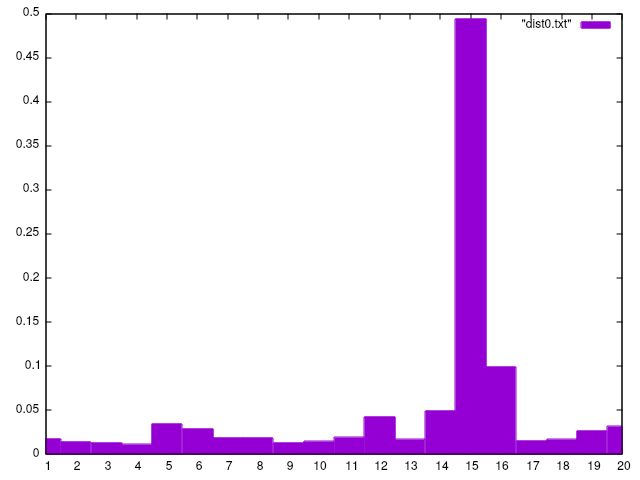
\includegraphics[scale=0.4]{dist0}
        \caption{ Distribución de las probabilidades en la primera iteración. }
      \end{minipage}
      \begin{minipage}{0.5\linewidth}
        \centering
        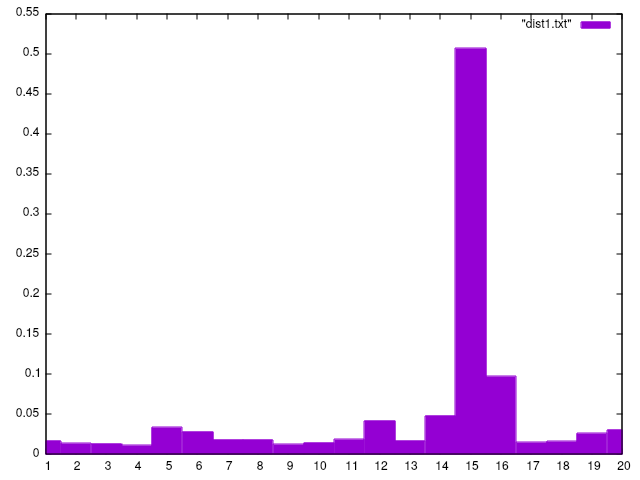
\includegraphics[scale=0.4]{dist1}
        \caption{ Distribución de las probabilidades a la mitad de las iteraciones. }
      \end{minipage}
      
      \begin{minipage}{\linewidth}
        \centering
        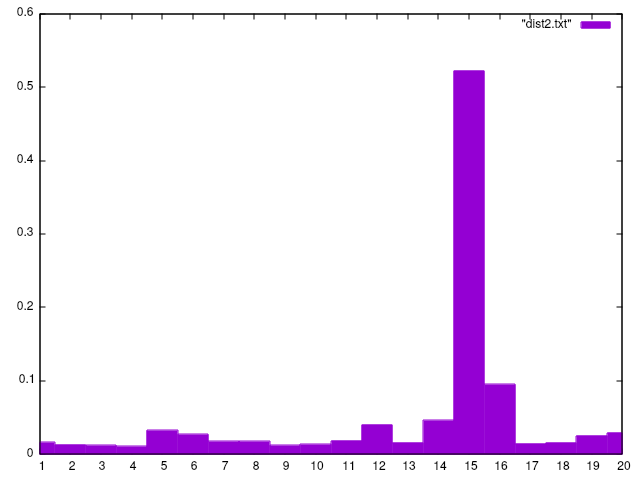
\includegraphics[scale=0.4]{dist2}
        \caption{ Distribución de las probabilidades en la última iteración. }
      \end{minipage}
    \end{figure}

    \section{Discusión} \label{discussion}
    De todos los experimentos que se realizaron, parece que 
    los parametros de la huerística no tienen un gran 
    impacto sobre los resultados que se obtienen. Todos los
    experimentos regresaron soluciones factibles pero 
    con costos algo elevados comparado con las soluciones 
    óptimas. Además de que podemos observar desde un principio
    en la distribución de las probabilidades que las hormigas 
    se van con el trabajador que pueda realizar la tarea 
    gastando la menor capacidad posible.

    Todo lo anterior, parece apuntar a que la huerística 
    funciona de una forma \tit{elitista} o \tit{glotona}
    en donde desde un principio busca a los mejores 
    candidatos basándose únicamente en su capacidad. 
    Resultando así en soluciones factibles pero nada 
    óptimas. Afortunadamente hay varias maneras de resolver
    este problema para futuros trabajos, uno de ellos
    podría ser agregar un factor de ``disipación''
    o ``distribución'', en donde en vez de que 
    $\eta$ regrese 0 en (\ref{n_update}), esta regrese la
    probabilidad original de escoger a esa arista
    multiplicada por este factor $\phi$ de ``distribución''.
    Así en un principio nuestras soluciones van a ser muy 
    malas y posiblemente no factibles, pero nos van a 
    permitir distribuir nuestras soluciones; de tal 
    forma que ya avanzada la huerística esta construya 
    soluciones factibles a partir de las 
    malas que había encontrado en un principio. 
    Solucionando así el que nos atoremos 
    en un mínimo local muy malo.

    \section{Conclusiones} \label{conclussion}
    La heurística de optimización de colonia de hormigas
    (ACO) resultó como una buena alternativa para 
    poder encontrar soluciones factibles al problema 
    de asignación generalizado (GAP). Cabe mencionar
    que posiblemente ACO también pueda encontrar
    soluciones factibles óptimas a GAP; sin embargo,
    en este trabajo se observó que también es 
    necesario permitir que nuestras hormigas 
    puedan explorar malas soluciones desde un principio,
    pues de lo contrario la heurística empezará a comportarse
    como un algoritmo glotón y se estancará en un 
    mínimo local posiblemente muy malo.

    Los parametros de la huerística no parecieron 
    tener un gran impacto sobre el rendimiento de la
    huerística, pero siempre es recomendable 
    mantener el número de hormigas reducido y 
    tener en cuenta la relación que existe entre las
    feromonas de la heurística y los valores 
    $\eta$ de la huerística; esta relación, al 
    final, es qué tanto difiere $\alpha$ de $\beta$.
    Esto último es importante, pues así podemos 
    definir qué va a tener más impacto 
    sobre las decisiones de las hormigas, si la 
    información que nos da la heurística desde un 
    prinicipio (las capacidades de los trabajadores
    para realizar una tarea) ó las feromonas que 
    han dejado las hormigas en anteriores iteraciones
    (los costos de las soluciones encontradas); balancear 
    estas dos le permitirá a nuestra hormigas encontrar
    mejores soluciones con las condiciones que deseamos.

    \section*{Bibliografía}
    
    \begin{itemize}
      \item O Erhun Kundakcioglu and Saed Alizamir. 
        Generalized assignment problem., 2009.
      \item Blum Christian. Ant Colony Optimization: 
        Introduction and Recent Trends. ELSEVIER. 2005.
      \item Dorigo Marco and Stützle Thomas.
        Ant Colony Optimization. The MIT PRESS. 2004.
    \end{itemize}
    
\end{document}
